\FloatBarrier
\subsection{Effects of initial conditions}
We adjusted the white noise output implementation from the preceding section to analyze the impact of initial values and conditions on system identification. Specifically, we varied the initial values for the $P$ matrix, which was previously defined as line 38 in \autoref{code:EICP}. The system's output and parameters, when using the original $P$ values, are presented in \autoref{fig:RLSIWNOWhiteNoiseOutput} and \autoref{fig:RLSIWNOWhiteNoiseParams}.

\begin{code}
	\begin{matlabcode}{firstnumber = 38}
        P{L}=eye(na+nb+1)*10^(6); %Usual P
		%P{L}=eye(na+nb+1)*10^(2); %Smaller P
		%P{L}=eye(na+nb+1)*10^(12); %Bigger P
	\end{matlabcode}
	\captionof{listing}{varying $P$}
	\label{code:EICP}
\end{code}

The impact of a smaller initial $P$ matrix on system parameter identification is illustrated in \autoref{fig:EICSmallerPParams}, while the effect of a larger initial $P$ matrix is shown in \autoref{fig:EICBiggerPParams}.

\begin{figure}
	\centering
	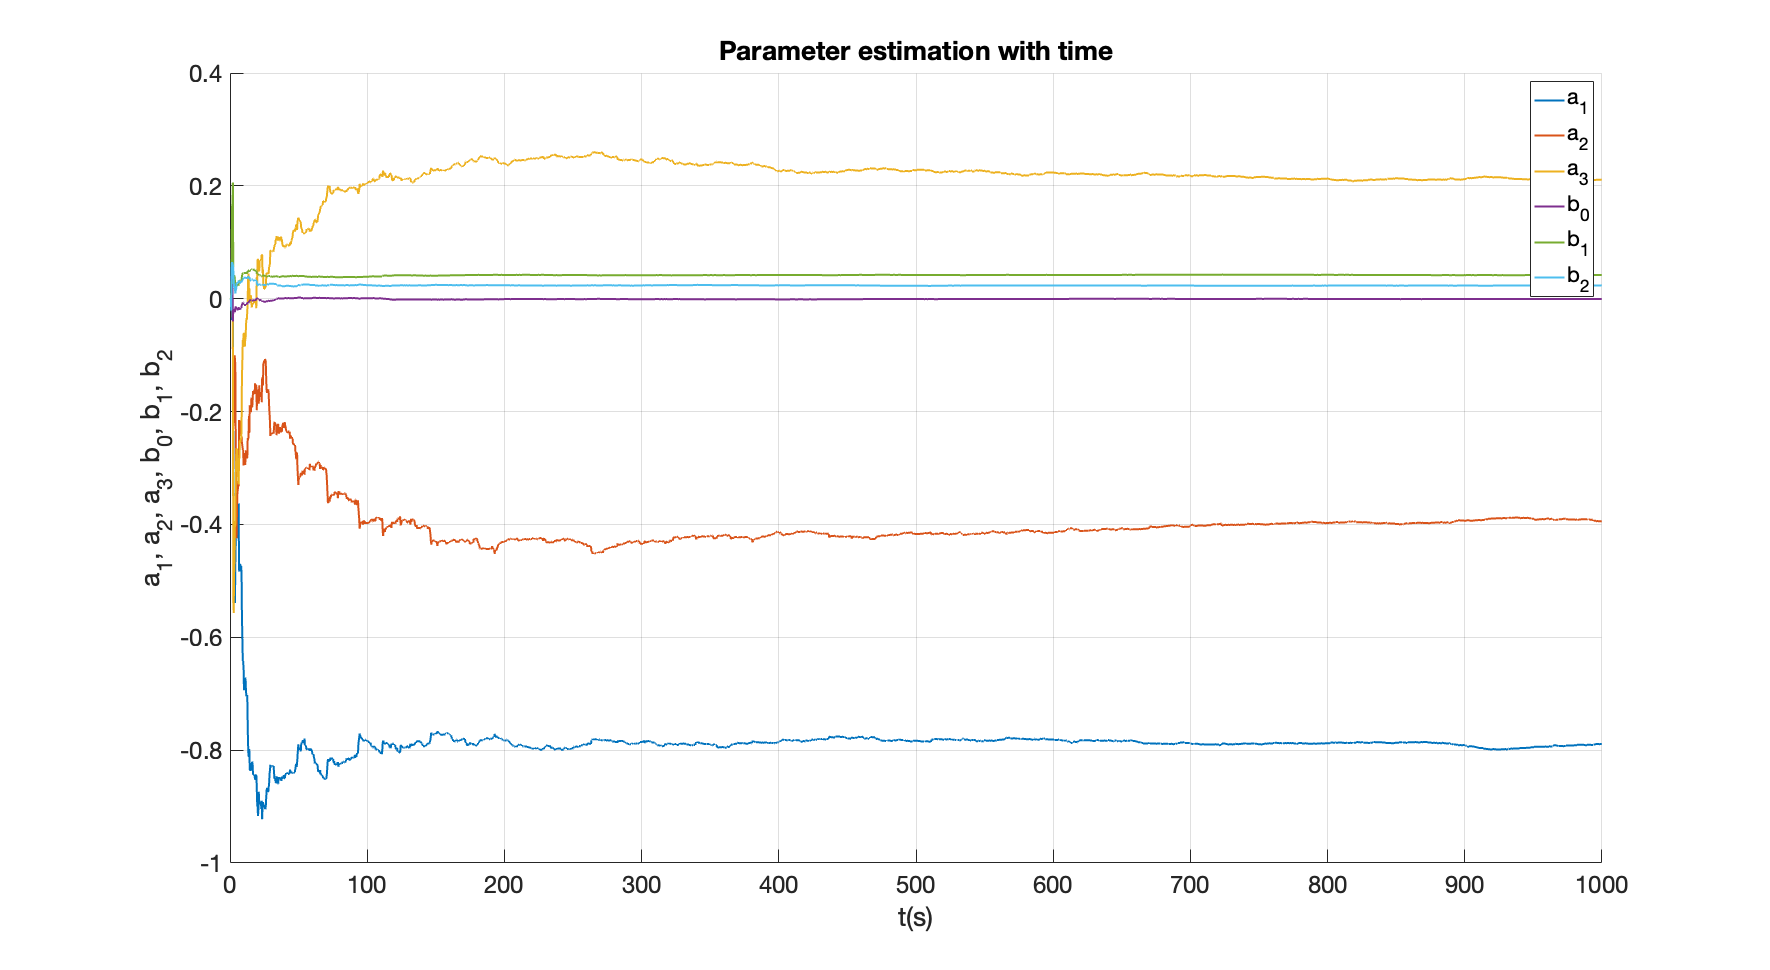
\includegraphics[totalheight=8cm]{images/EICSmallerPParams.png}
	\caption{System parameters with smaller $P$}
	\label{fig:EICSmallerPParams}
\end{figure}

\begin{figure}
	\centering
	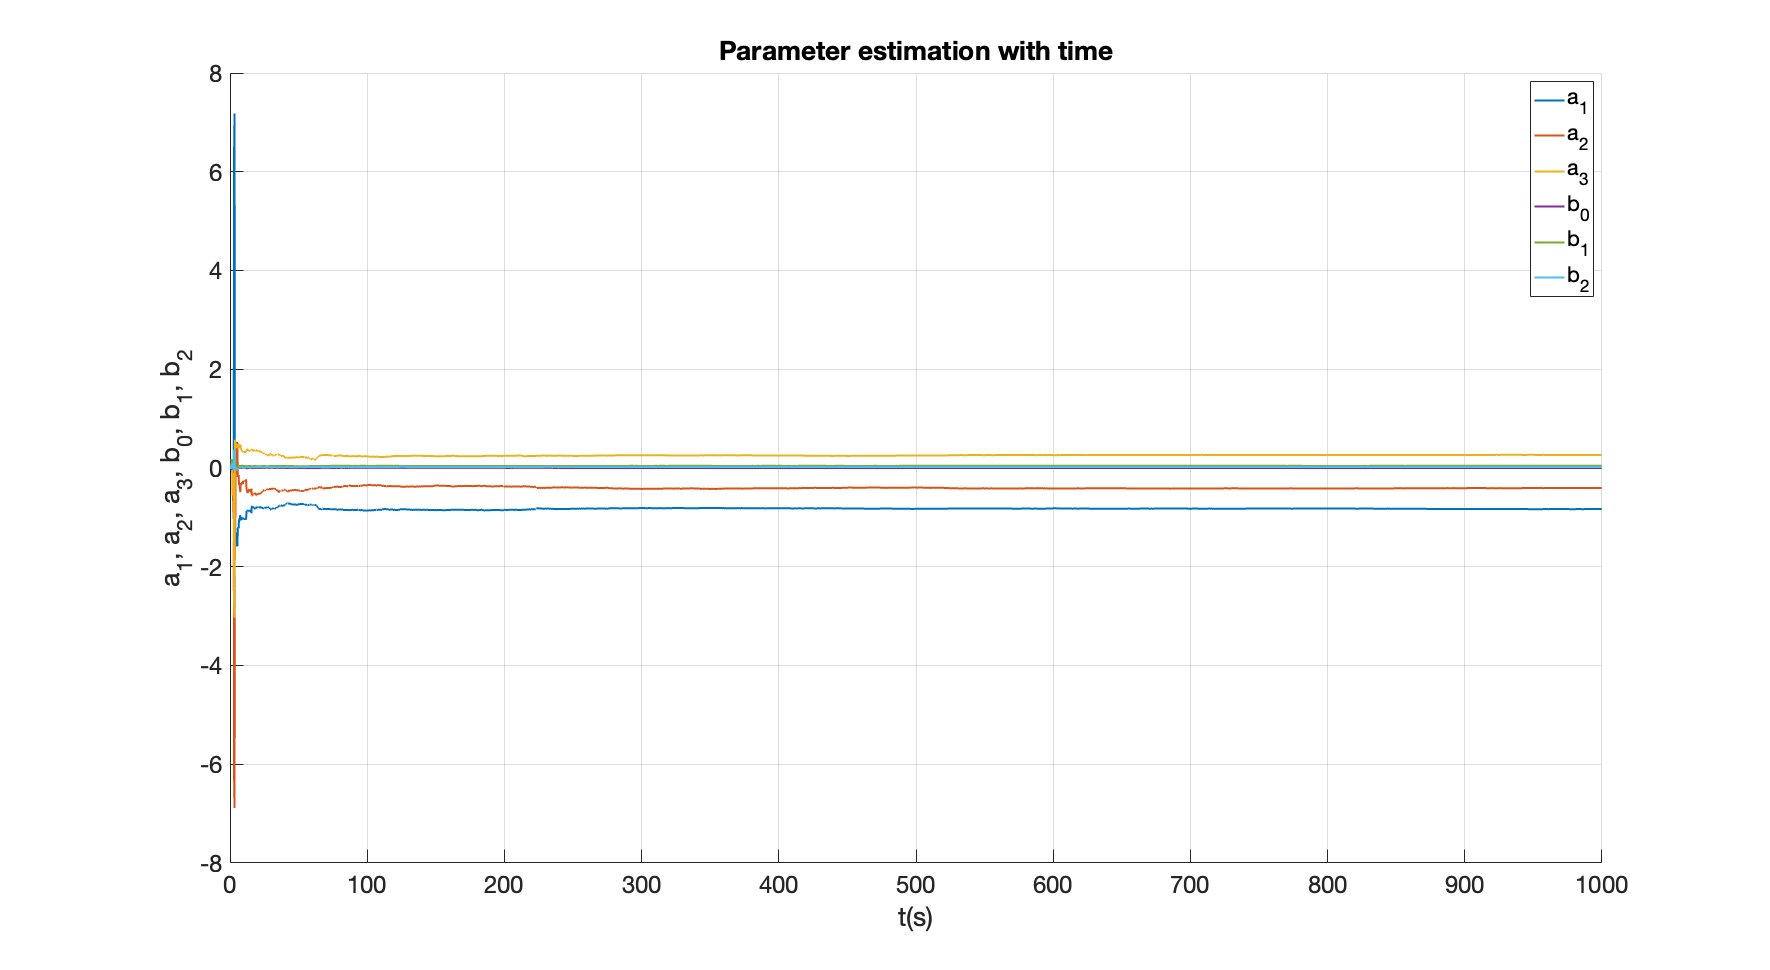
\includegraphics[totalheight=8cm]{images/EICBiggerPParams.png}
	\caption{System parameters with bigger $P$}
	\label{fig:EICBiggerPParams}
\end{figure}

Matlab code for varying the amount of initial $P$ values is located at   \hspace{-1ex}\lstinline| assignment1/part2/2_3/RLS2_3_vary_P.m|.


Additionally, we explored the impact of varying the initial $\theta$ values. The effect of using initial $\theta$ values closer to the actual values is shown in \autoref{fig:EICBetterThetaParams}, while the results of intentionally using less accurate initial $\theta$ values are presented in \autoref{fig:EICWorseThetaParams}.

\begin{code}
	\begin{matlabcode}{firstnumber = 38}
for i=1:N
theta_hat(:,i)=[-0.79;-0.41;0.23;-0.0009;0.042;0.022]; %Better Theta
%theta_hat(:,i)=[100;100;100;100;100;100]; %Worse Theta
end
	\end{matlabcode}
	\captionof{listing}{varying $\theta$}
	\label{code:EICTheta}
\end{code}

\begin{figure}
	\centering
	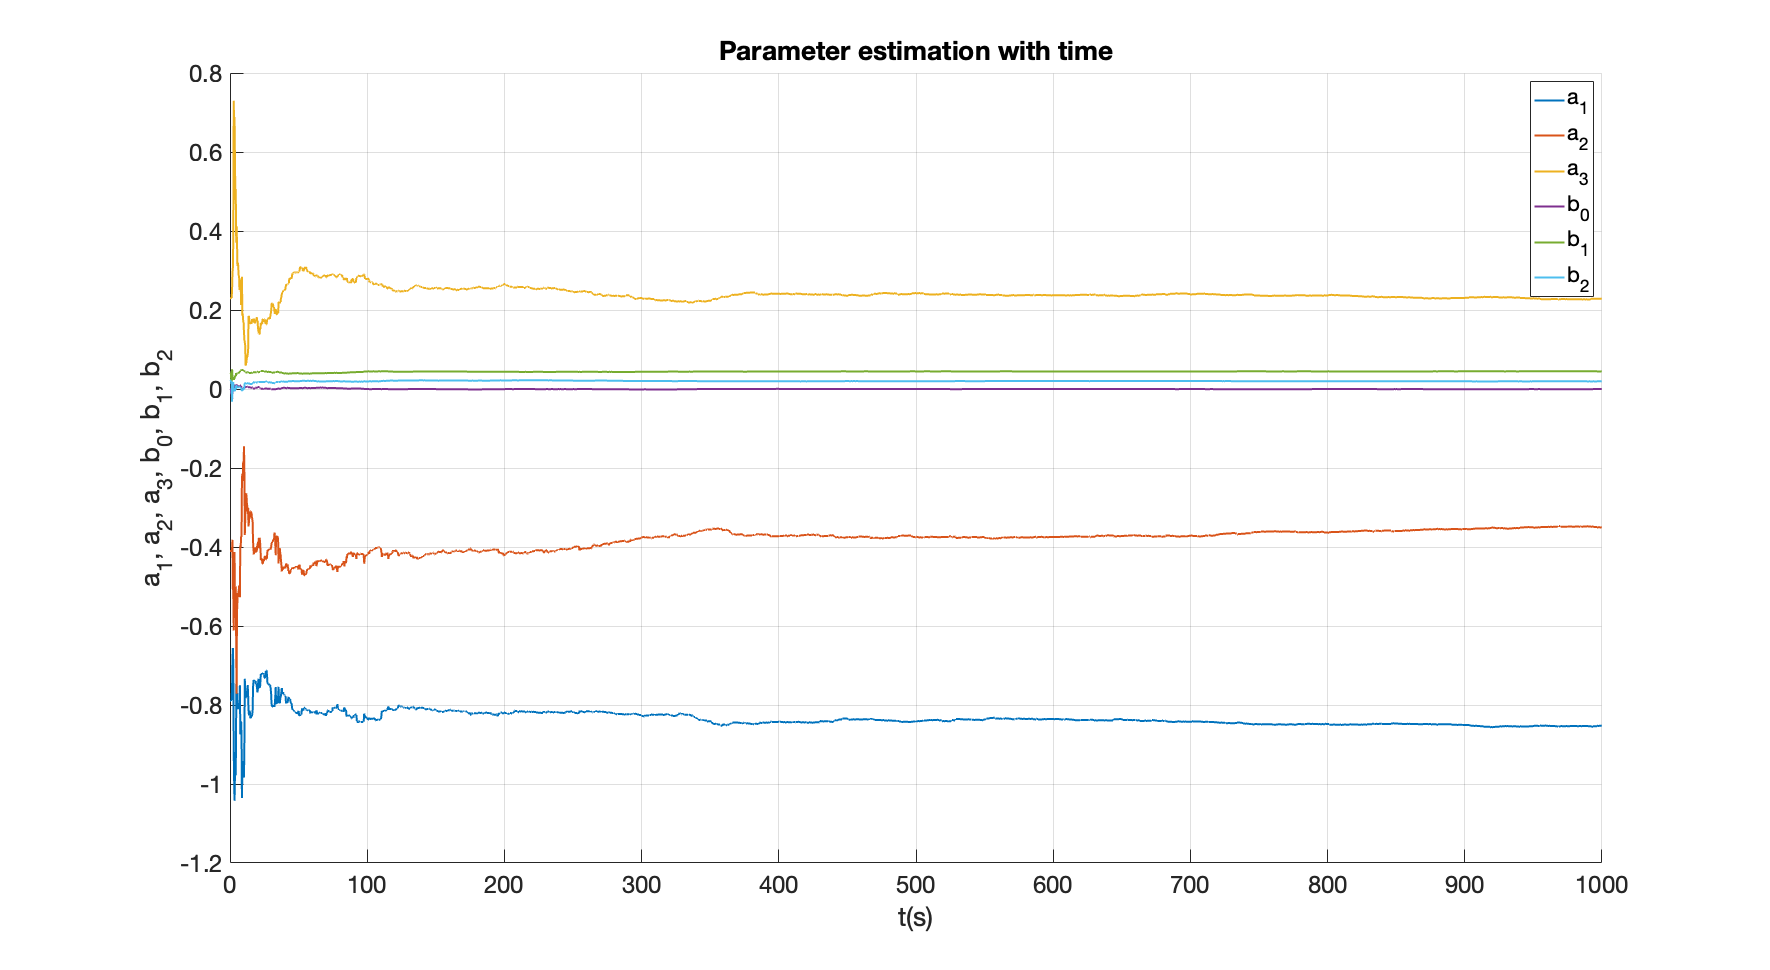
\includegraphics[totalheight=8cm]{images/EICBetterThetaParams.png}
	\caption{System parameters with better initial $\theta$}
	\label{fig:EICBetterThetaParams}
\end{figure}

\begin{figure}
	\centering
	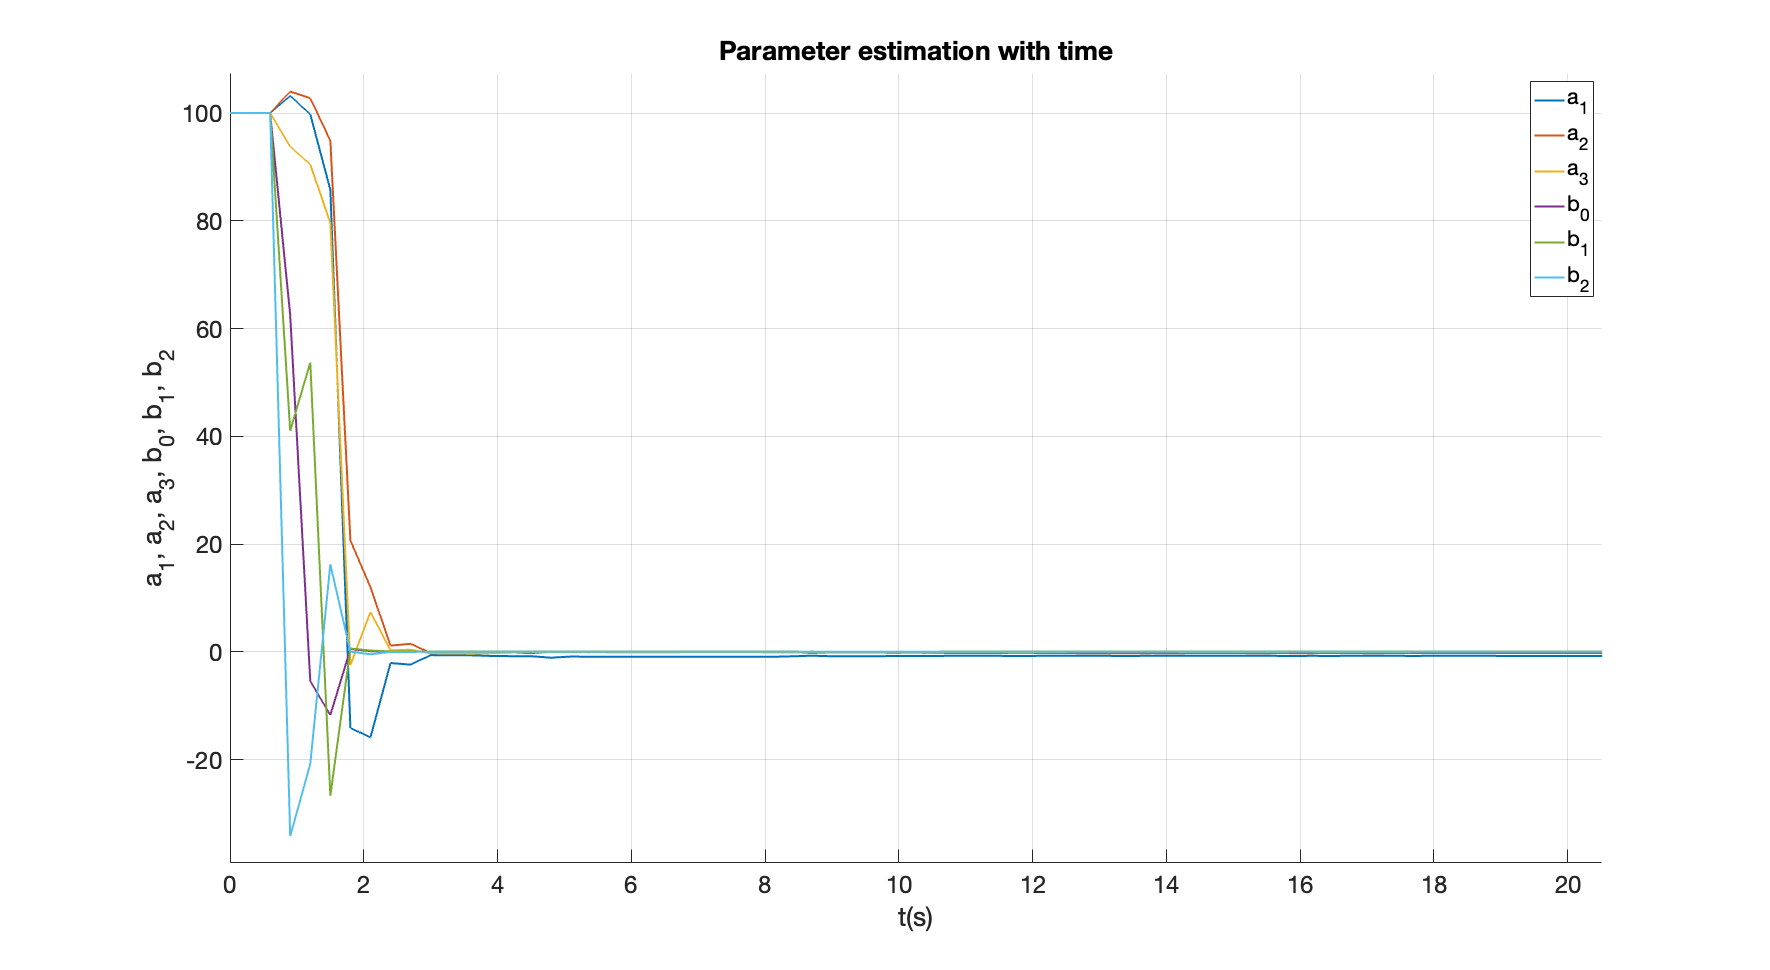
\includegraphics[totalheight=8cm]{images/EICWorseThetaParams.png}
	\caption{System parameters with worse initial $\theta$}
	\label{fig:EICWorseThetaParams}
\end{figure}

Matlab code for varying the amount of initial $\theta$ values is located at   \hspace{-1ex}\lstinline| assignment1/part2/2_3/RLS2_3_vary_theta.m|.
